\documentclass{article}
\usepackage{graphicx} % Required for inserting images

\title{Math 496 the solution of $x! = x ^ {t}$ and its variants}
\author{Haotian Ju, Saibo Xu}
\date{May 2023}
%\documentclass{article}
\usepackage{graphicx}
\usepackage{amsmath}
\usepackage{amsfonts}
\usepackage{amssymb}
\usepackage{amsthm}
\usepackage{parskip}
\usepackage{ulem}
\usepackage{tikz}
\usepackage{graphicx}
\usepackage{csquotes}
\usepackage[pdfusetitle]{hyperref}
\begin{document}
\maketitle
        \tableofcontents
        \newpage
        \section{Introduction}
        The main topic for this paper is to discuss the solutions of the equation $x! = x ^ {t}$ and its variants. The methods to approximate the solutions can be various. For example, some algorithms can be used on this equation to approximate the solution. Moreover, we can use some theorems and lemmas in number theory to find an accurate solution. In this paper, the main function that will be used is some number theory theorems together with some knowledge of gamma functions to deal with situations where $x$ is a decimal number. Also, we will use Stirling Approximation to simplify the equation.

        \section{Abstract}
        We can divide this whole problem into several categories. The first one, also the easiest one to work with is the situation when $x$ is a positive integer number. The second situation is when $x$ is a negative integer number. The third situation is when $x$ is a positive decimal number. The last one, also the most complicated one to work on, is when $x$ is a negative decimal number. This paper will show all the solutions to those 4 different situations in the order above. This paper will also show some variants of this problem so that it will have a wider range of applications to some future problems in number theory and other areas.

        \section{The uniqueness of the solution when $x$ and t are positive integer numbers}
        Before we go on to find the solution, we need to make sure that the solution actually exists, which means that there is at least one solution for this equation. We can rewrite this problem as\\
            \begin{align*}
                x! - x ^ {t} = 0
            \end{align*}\\
        to help us better find the solution in N.\\

        One root we can find to satisfy the requirement above is when $x$ = 1. We can easily prove it by bringing $x$ = 1 back to the original equation and getting the left-hand side and right-hand size equal to each other. \\

        To find other positive integer number solutions, we can use the graphing calculator to help us find regions where the solution may exist.\\


        \newpage
        \begin{figure}[h]
        \centering
        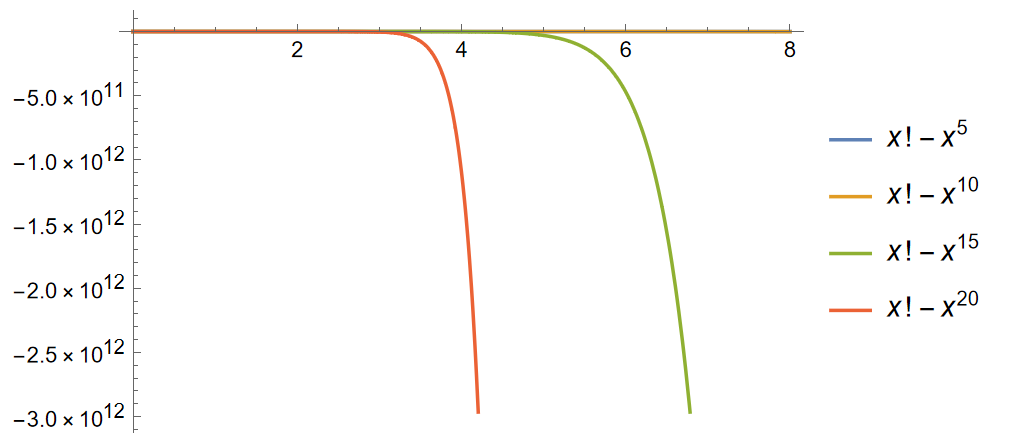
\includegraphics[width=8cm]{301.png}
        \caption{The graph of $f(x) = x! - x ^{t}$ for variant t values, where t is 5,10,15,20 by the order}
    
        \end{figure}

        The graph shows that the curve intersects with y = 0 on $x$ = 1 and another point. So, we need to do 2 things.\\

        1. We need to consider whether the second intersection point's $x$ part is an integer or not.\\
        2. We need to consider whether there are any other intersection points after the second intersection point.\\

        To better help us with the uniqueness problem, we can generate all the values for the $f(x) = x! - x^{t}$ corresponding to different t values to find a trend for the second intersection point as t increases.

        Next, we need to prove that there are no integer values greater than the second intersection point's $x$ part that can make $x! - x ^ {t}$ to 0.

        If n is an integer and $x! = x^t$, we consider when $x$ = 1, for all t belongs to integer set, x = 1 will be a solution for the $x! = x^t$.\\

        Next, for $x$ = 2, we can rewrite this formula to:
            \begin{align*}
                2! = 2^t
            \end{align*}\\
        Then, $2 = 2^t$, so t is 1.\\

        Finally, for $x$ greater than 2, there is no integer t such that $x! = x^t$, since $x$ - 1 $>$ 1 is a divisor of $x$! but $gcd(x-1, x) = 1.$
        
        \section{Approximate solution of the equation when $x$ is a positive number}
        When $x$ is not an integer number, we can use factorials to the $x!$ part. In this situation, we need to use the gamma function to compute the value of $x!$. 

        Definition(Gamma Function): The gamma function is defined for all complex numbers except the non-positive integers. For every positive integer n,
            \begin{align*}
                \Gamma(n) = (n - 1)!
            \end{align*}

        Derived by Daniel Bernoulli, for complex numbers with a positive real part, the gamma function is defined via a convergent improper integral:
            \begin{align*}
                \Gamma(n) = \int_0^\infty t^{n-1} e^{-t} dt 
            \end{align*}

        Since this function is hard to compute, we can find its approximation by using the Stirling Approximation:

        In mathematics, Stirling's approximation (or Stirling's formula) is an approximation for factorials. It is a good approximation, leading to accurate results even for small values of n. It is named after James Stirling, though a related but less precise result was first stated by Abraham de Moivre.\\
        One way of stating the approximation involves the logarithm of the factorial:\\

            \begin{align*}
                \ln(n!) = n * \ln(n) - n + \mathcal{O}(f(n))
            \end{align*}

        where the big O notation means that, for all sufficiently large values of n, the difference between $\ln(n!)$ and $n * \ln(n) - n$ will be at most proportional to the logarithm.\\

        In this paper, we use the simplest version of Stirling's formula, the derivation is:
            \begin{align*}
                \ln(n!) = \sum_{j=1}^{n} \ln(j)
            \end{align*}
        
        with an integral:\\
            \begin{align*}
                \sum^{n}_{j = 1} \ln(j) \approx  \int_{1}^{n} lnx \,dx = n * \ln(n) - n + 1
            \end{align*}\\
        
        We can use Stirling approximation to find the approximate solution of the equation $x! = x ^ {t}$.
        we take $log_e$ to both sides of the equation and got:
            \begin{align*}
                \ln(x!) = t * \ln(x)
            \end{align*}\\
        Then, we move the $\ln(x)$ to the left-hand side, and the equation then becomes,
            \begin{align*}
                t = \frac{\ln(x!)}{\ln(x)}
            \end{align*}\\
        Now, we can proceed with this formula and give a rough range for $t$:
        \begin{align*}
                t = \frac{\ln(x!)}{\ln(x)} = \frac{\ln{(x-1)!}+\ln x}{\ln x}=\frac{\ln{(x-1)!}}{\ln x}+1
        \end{align*}\\
        With the assistance of graphs, we can find that the function $\frac{\ln{(x-1)!}}{\ln x}$ is constantly greater than $0$ when $x$ is greater than the zero point $x=1$. Therefore, for $x>1$, $t>1$. However, for $x<1$, the value of the function goes more complicated. 
        Here, we need to do some approximation of $\ln(x!)$ to help us further find the solution.\\

        \begin{figure}[h]
        \centering
        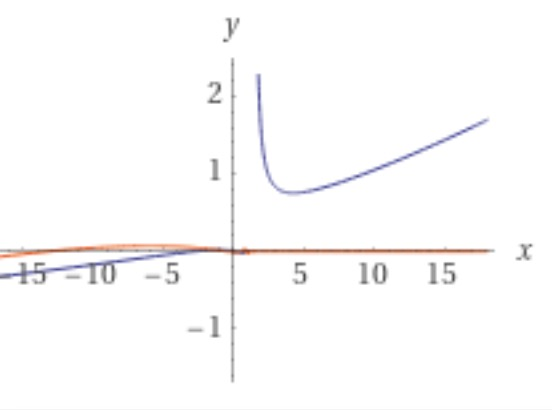
\includegraphics[width=12cm, height = 5cm]{101.jpg}
        \caption{Graph for $y = \frac{\ln(x-1)!}{\ln(x)}$}
        \label{fig:picture}
        \end{figure}

        \begin{figure}[h]
        \centering
        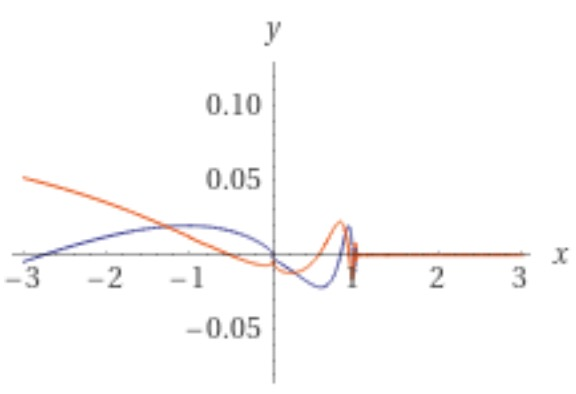
\includegraphics[width=12cm, height = 5cm]{102.jpg}
        \caption{Graph for $y = \frac{\ln(x-1)!}{\ln(x)}$}
        \label{fig:picture}
        \end{figure}
        
        Therefore, we can use $n * \ln(n) - n + 1$ to approximate $\ln(n!)$, then the equation becomes:
            \begin{align*}
                t \approx \frac{x * \ln(x) - x + 1}{ln(x)}
            \end{align*}\\
        Expand the right-hand side and the equation becomes:
            \begin{align*}
                t \approx x - \frac{x}{\ln(x)} + \frac{1}{\ln(x)}
            \end{align*}\\

        Then, to find the approximate solution of $x! = x^{t}$, we need to solve the equation above. What's more, if we want the equation to have a solution at $x = \alpha$, we can directly bring this solution to the right-hand side of the equation, and we got:
            \begin{align*}
                t \approx \alpha - \frac{\alpha}{\ln(\alpha)} + \frac{1}{\ln(\alpha)}
            \end{align*}\\

        From figure 4, we can see a trend that as the t increases, the second solution also increases. To prove this theorem, we can graph the function above to help us better understand the problem. we can see that the function intersection with the x-axis at $x$ = 0. In the original function $x! = x^t$, if we bring the t = 0 back, we can see that the only solution is at $x$ = 0.\\

        

        \begin{figure}
        \centering
        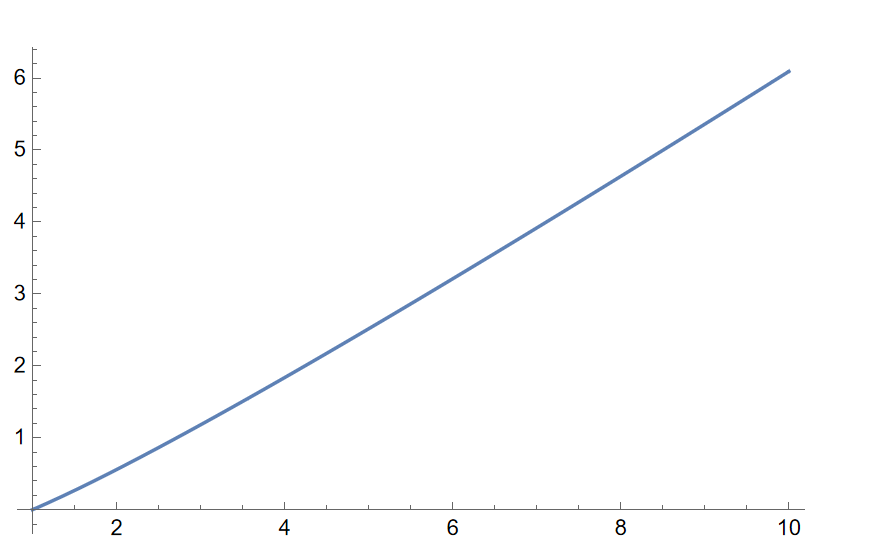
\includegraphics[width=8cm, height=5cm]{302.png}
        \caption{The graph of the function $t = \frac{x * \ln(x) - x + 1}{\ln(x)}$}
        \end{figure}

        \newpage
        We set the domain of the $x$ to be all the real values greater than 0:\\
        Next, we need to take the derivative of the $t = \frac{x * \ln(x) - x + 1}{\ln(x)}$, which is:\\
            \begin{align*}
                \frac{dt}{dx} = \frac{d}{dx} \frac{x * \ln(x) - x + 1}{\ln(x)}
            \end{align*}
        This is equal to:\\
            \begin{align*}
                \frac{dt}{dx} = \frac{x(\ln(x) ^ 2 - \ln(x) + 1) - 1}{x(\ln(x) ^ 2)}
            \end{align*}
        From Figure 5, we can see that:\\
        
            
            \begin{figure}[h]
            \centering
            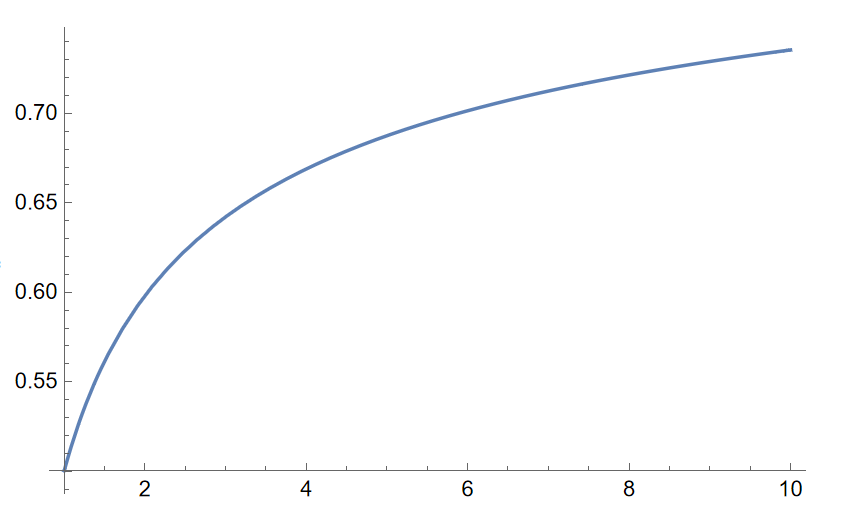
\includegraphics[width=8cm, height=4cm]{303.png}
            \caption{The graph of the function $\frac{dt}{dx} = \frac{x(\ln(x) ^ 2 - \ln(x) + 1) - 1}{x(\ln(x) ^ 2)}$}
            \end{figure}
        So we can see that as $x$ increases, t also increases.\\

        Next, we use a well-known theorem to find the trend of $\frac{dx}{dt}$:\\
        Inverse Function Theorem: Let f($x$) be a function that is both invertible and differentiable. Let  $y = f^{-1}(x)$ be the inverse of f(x). For all  x satisfying  $f^{'}(f^{-1}(x)) \neq 0$,
            \begin{align*}
                \frac{dy}{dx} = \frac{d}{dx} (f^{-1}(x)) = (f^{-1})^{'}(x) = \frac{1}{f^{'}(f^{-1}(x))}
            \end{align*}
        Alternatively, if  y=g($x$) is the inverse of  f($x$), then
            \begin{align*}
                g^{'}(x) = \frac{1}{f^{'}(g(x))}
            \end{align*}
        We define $x$ = g(t), which is the inverse function of f($x$).\\
        Then, from Figure 3, we can see that for every $x > 1$, the derivative $\frac{dx}{dt}$ is greater than 0, and t is also greater than 0 for all $x > 1$. We can also see that when $t > 0$, $x > 1$. Therefore, the g(t) will stay positive for every t > 0. Since when $x > 0$, $f^{'}(x)$ is greater than 0, then $\frac{1}{f^{'}(g(t))}$ should be also greater than 0. Thus, $g^{'}(t)$ will be positive for all t greater than 0. \\

        After we proved this, we can say that as the t increases, then the $x$ value of the second solution of the equation $x! = x ^ {t}$ will increase as well.

        \subsection{Another approach for the problem}
        Another approach would be to make a table of $\ln(x!)/(\ln x)$ for various values of $x$ and make an estimate for this as a function of $x$. Here we will use the Sterling formula for this problem\\
        We use the $log_e(x)$ for all the $\log()$ functions.\\
        
        \begin{tabular}{c c}
        % The table content goes here
        $x$ = 1 & log($x$!)/(log $x$) = 1 \\
        $x$ = 5 & log($x$!)/(log $x$) = 2.9746358687061645 \\
        $x$ = 10 & log($x$!)/(log $x$) = 6.559763032876793 \\
        $x$ = 20 & log($x$!)/(log $x$) = 14.131975956091887 \\
        $x$ = 30 & log($x$!)/(log $x$) = 21.950574451031976 \\
        $x$ = 40 & log($x$!)/(log $x$) = 29.906274001912664 \\
        $x$ = 50 & log($x$!)/(log $x$) = 37.95421620623191 \\
        $x$ = 100 & log($x$!)/(log $x$) = 78.98500182735788 \\
        $x$ = 200 & log($x$!)/(log $x$) = 162.92568516989743 \\
        $x$ = 500 & log($x$!)/(log $x$) = 420.19229806673394 \\
        \end{tabular}\\
        So, we can see an increasing trend for the t as we would like to have an intersection point for ($x$, $y$ = 0).\\

        Therefore, we can make the assumption that as the intersection point for $x$ increases, t will also increase. To make a good estimation of t for any given $x$, we use Sterling Theorem to expand the log($x$!).\\

        \newpage
        
        For the equation $\frac{\ln(x!)}{x\ln(x)}$, we can see that its value approaches 1 as we increase the values of x. We can see this from the graph: \\ 


            \begin{figure}[h]
                \centering
                
\includegraphics[width=8cm, height=1cm]{201.png}
                \caption{The code for the function $\frac{\ln(x!)}{x\ln(x)}$ with $x$ ranges from 1 to 10000000000000}
                \end{figure}
            
            \begin{figure}[h]
                \centering
                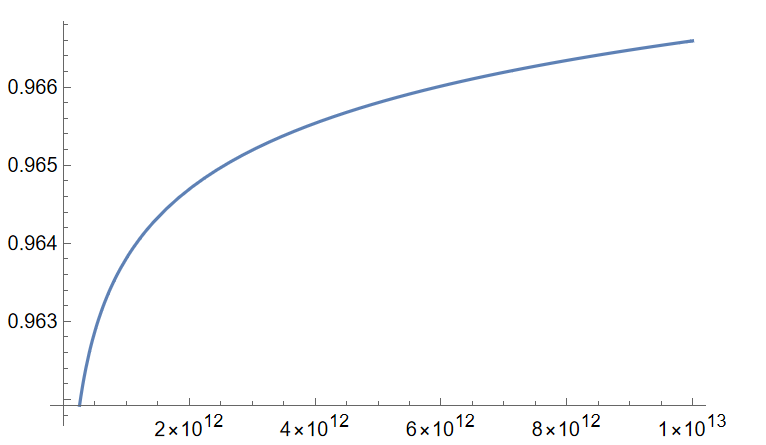
\includegraphics[width=8cm, height=5cm]{202.png}
                \caption{The graph of the function $\frac{\ln(x!)}{x\ln(x)}$}
                \end{figure}

        To mathematically prove it, we need to use the Stirling again.
            \begin{align*}
                \frac{\ln(x!)}{x\ln(x)} \approx \frac{x \ln(x) - x + 1}{x \ln(x)}
            \end{align*}
        which can be written into:
            \begin{align*}
                \frac{\ln(x!)}{x\ln(x)} \approx 1 - \frac{1}{\ln(x)} + \frac{1}{x\ln(x)}
            \end{align*}
        So as the x increases, the latter 2 terms approach 0. Therefore the whole equation approaches 1 as x is big enough.
        \section{Lower bound and Upper bound of the solutions for $x! = x ^ {t}$ }
        In this problem, We can use the formula for n! is in the range of:
            \begin{align*}
                (\sqrt{2\pi n} (\frac{n}{e})^n e^{\frac{1}{12n+1}},\sqrt{2\pi n} (\frac{n}{e})^n e^{\frac{1}{12n}})
            \end{align*}
        Then, we bring this range back to the equation:\\
            \begin{align*}
                t = \frac{ln(x!)}{ln(x)}
            \end{align*}
        To find the lower bound and upper bound for the solution of $x! = x^t$.\\

        $ln(x!)$ is in the range of:
            \begin{align*}
                (ln(\sqrt{2\pi x} (\frac{x}{e})^x e^{\frac{1}{12x+1}}),ln(\sqrt{2\pi x} (\frac{x}{e})^x e^{\frac{1}{12x}}))
            \end{align*}
        And then, t is in the range of:\\
            \begin{align*}
                (\frac{ln(\sqrt{2\pi x} (\frac{x}{e})^x e^{\frac{1}{12x+1}})}{ln(x)},\frac{ln(\sqrt{2\pi x} (\frac{x}{e})^x e^{\frac{1}{12x}})}{ln(x)})
            \end{align*}
        Therefore, for a fixed t, to find an interval of $x$ where the solution is sure to exist, we need to solve the $x$ for both of the equations to find the lower bound and upper bound of the interval.
        So, the lower bound and upper bound of the interval can be solved by the 2 equations below:
            $$\left\{\begin{matrix}
            &\frac{ln(\sqrt{2\pi x} (\frac{x}{e})^x e^{\frac{1}{12x+1}})}{ln(x)} - t = 0, \text{ (1)} \\ 
            & \frac{ln(\sqrt{2\pi x} (\frac{x}{e})^x e^{\frac{1}{12x}})}{ln(x)} - t = 0, \text{ (2)} 
        \end{matrix}\right.$$

        Next, for some given t value, we can see the intervals where the solutions are sure to exist: \\
        \section{Some changes for the form of the equation $x! = x ^ {t}$ but still the same problem}
        \subsection{The approximate solution for $(\alpha x)! = (\alpha x) ^ t$}
        Suppose that we substitute $x$ to $\alpha x$, then we try to find the approximate solution for this new equation. In this problem, we can still use the methods above to find the approximate solution.\\

        For the first step of the solution, we take $log_e$ for both sides, then we have:
            \begin{align*}
                \ln((\alpha x)!) = t * \ln(\alpha x)
            \end{align*}
        Then, we rewrite the formula as:
             \begin{align*}
                t = \frac{\ln((\alpha x)!)}{\ln(\alpha x)}
            \end{align*}
        At this time, to simplify the computation, we define $y$ = $\alpha x$, so that:
            \begin{align*}
                t = \frac{ln(y!)}{ln(y)}
            \end{align*}
        Therefore, we can expand $\ln(y!)$ to:
            \begin{align*}
               \ln(y!) \approx y * \ln(y) - y + 1
            \end{align*}
        So that the t can be written as an equation of $y$:
            \begin{align*}
               t \approx \frac{y * \ln(y) - y + 1}{\ln(y)} = y - \frac{y}{\ln(y)} + \frac{1}{\ln(y)}
            \end{align*}
        Next, we bring $y$ = $\alpha x$ back to the equation above and get:
            \begin{align*}
               t \approx \alpha x - \frac{\alpha x}{\ln(\alpha x)} + \frac{1}{\ln(\alpha x)}
            \end{align*}
        In this problem, we can still find the lower bound and upper bound for the solution x corresponding to given t:\\
        \subsection{The approximate solution for $(\alpha x)! = (\alpha x) ^ {\beta t}$}
        Next, we more generalize the original equation by substituting the t to $\beta t$, where $\beta$ $\in$ $\mathbb{R}$. 

        We still take $\ln$ to both sides, and we get:
            \begin{align*}
               \ln((\alpha x)!) = \beta t\ln(\alpha x)
            \end{align*}
        Therefore, t is equal to:
            \begin{align*}
               t = \frac{\ln((\alpha x)!)}{\beta \ln(\alpha x)}
            \end{align*}
        We use the Sterling formula to expand $\ln((\alpha x))!$:
            \begin{align*}
                \ln(\alpha x!) \approx \alpha x * \ln(\alpha x) - \alpha x + 1
            \end{align*}
        Therefore, we got the solution for t:
            \begin{align*}
                t \approx \frac{\alpha x}{\beta} - \frac{\alpha x}{\beta \ln(\alpha x)} + \frac{1}{\beta \ln(\alpha x)}
            \end{align*}
        This is only an approximate solution for t given the value of $x$. We can find a region where an accurate solution is sure to exist.\\

        We still use this region for n! to solve the problem:
            \begin{align*}
                (\sqrt{2\pi n} (\frac{n}{e})^n e^{\frac{1}{12n+1}},\sqrt{2\pi n} (\frac{n}{e})^n e^{\frac{1}{12n}})
            \end{align*}
        This can be used to find the interval of t:
            \begin{align*}
               t \in (\frac{ln(\sqrt{2\pi \alpha x} (\frac{\alpha x}{e})^{\alpha x} e^{\frac{1}{12(\alpha x)+1}})}{ln(\alpha x)},\frac{ln(\sqrt{2\pi \alpha x} (\frac{\alpha x}{e})^{\alpha x} e^{\frac{1}{12(\alpha x)}})}{ln(\alpha x)})
            \end{align*}
        Therefore, if we want a solution at $x$, we can bring this value back to the interval above, and there exists a t such that the equation holds for given $\alpha$ and $\beta$. 

        \section{Some variants of the equation $x! = x ^ {t}$}
        \subsection{The approximate solution of $x! = (\alpha x) ^ {t}$}
        we still take $\ln$ to both sides, then we got:
            \begin{align*}
               \ln(x!) = t * \ln(\alpha x)
            \end{align*}
        Then, we use Stirling approximation to rewrite the equation:
            \begin{align*}
               x * \ln(x) - x + 1 \approx t * \ln(\alpha x)
            \end{align*}
        Therefore, we got t as an equation of x:
            \begin{align*}
               t \approx \frac{x * \ln(x) - x + 1}{\ln(\alpha) + \ln(x)}
            \end{align*}
        From this equation, if we assume that there is a solution at the point $x = \beta$, we can use the equation above to find the approximated t corresponding to the $x = \beta$:
            \begin{align*}
               t \approx \frac{\beta * \ln(\beta) - \beta + 1}{\ln(\alpha) + \ln(\beta)}
            \end{align*}
        We can compare $x! = (\alpha x) ^ {t}$ with $x! = x ^ {t}$, if we would like to find the "t"s corresponding to $x = \beta$ for both of the equations. There should be a difference between those 2 equations:\\
            \begin{align*}
                \left\{\begin{matrix}
                    & \beta! = \beta ^ {t}\text{(1)} \\ 
                    & \beta! = (\alpha * \beta) ^ {t}\text{(2)} 
                \end{matrix}\right.
            \end{align*}

        We solve for t for both equations and get:
            \begin{align*}
               \left\{\begin{matrix}
                    & t_1 = \frac{\ln(\beta !)}{\ln(\beta)} \text{(1)} \\ 
                    & t_2 = \frac{\ln(\beta !)}{\ln(\beta) + \ln(\alpha)} \text{(2)} 
                \end{matrix}\right.
            \end{align*}

        Then, we rewrite $t_2$ to a function contains $t_1$:
            \begin{align*}
                t_2 = \frac{\ln(\beta !)}{\ln(\beta)} * \frac{\ln(\beta)}{\ln(\beta) + \ln(\alpha)}
            \end{align*}
        Where the first term is $t_1$, so:
            \begin{align*}
                t_2 = t_1 * \frac{\ln(\beta)}{\ln(\beta) + \ln(\alpha)}
            \end{align*}
        For the second term, we can rewrite it as:
            \begin{align*}
                \frac{\ln(\beta)}{\ln(\beta) + \ln(\alpha)} = 1 - \frac{\ln(\alpha)}{\ln(\beta) + \ln(\alpha)}
            \end{align*}
        Therefore, $t_2$ is equal to:
            \begin{align*}
                t_2 = t_1 * (1 - \frac{\ln(\alpha)}{\ln(\beta) + \ln(\alpha)})
            \end{align*}
        The term $1 - \frac{\ln(\alpha)}{\ln(\beta) + \ln(\alpha)}$ will reach to 0 if we take $\beta$ big enough. Therefore, $t_2$ will be closer and closer to $t_1$ if we increase the value of $\beta$

        
        \subsection{The approximate solution of ${(\alpha x)}! = x ^ {t}$}
        We still try to use the Stirling function to solve this problem\\

        We take $ln$ for both sides and got:
            \begin{align*}
                \ln((\alpha x)!) = t * \ln(x)
            \end{align*}
        Then we can rewrite t as a function of x:
            \begin{align*}
                t = \frac{\ln((\alpha x)!)}{\ln(x)}
            \end{align*}
        Since we have $\ln(x!) \approx x * \ln(x) - x + 1$, we can write t as:
            \begin{align*}
                t \approx \frac{\alpha * x * \ln(\alpha * x) - \alpha * x + 1}{\ln(x)}
            \end{align*}
        Next, we rewrite the equation as:
            \begin{align*}
                t \approx \frac{\alpha * x * (\ln(x) + \ln(\alpha)) - \alpha * x + 1}{\ln(x)}
            \end{align*}
        Then, t is equal to:
            \begin{align*}
                t \approx \alpha * x * \frac{\ln(x) - \ln(\alpha) + 1}{\ln(x)} + 1
            \end{align*}
             
        We can also consider the upper and lower bound for t as we assume $x$ to be a fixed point:\\

        From the formulas above, we have:
            \begin{align*}
                x! \in (\sqrt{2\pi x} (\frac{x}{e})^x e^{\frac{1}{12x+1}},\sqrt{2\pi x} (\frac{x}{e})^x e^{\frac{1}{12x}})
            \end{align*}
        And,
            \begin{align*}
                \ln(x!) \in (ln(\sqrt{2\pi x} (\frac{x}{e})^x e^{\frac{1}{12x+1}}),ln(\sqrt{2\pi x} (\frac{x}{e})^x e^{\frac{1}{12x}}))
            \end{align*}
        Which is equal to:
            \begin{align*}
               \ln(x!) \in ((\frac{1}{12x+1} - x)\ln(\sqrt{2 \pi x} * x^x),(\frac{1}{12x} - x)\ln(\sqrt{2 \pi x} * x^x))
            \end{align*}
        So the $\ln(\alpha x)$ is in the range of:
            \begin{align*}
               \ln(\alpha x!) \in ((\frac{1}{12(\alpha x)+1} - \alpha x)\ln(\sqrt{2 \pi \alpha x} * (\alpha x)^{\alpha x}),(\frac{1}{12(\alpha x)} - \alpha x)\ln(\sqrt{2 \pi \alpha x} * (\alpha x)^{\alpha x}))
            \end{align*}
        Finally, we bring the interval back to the equation, and we have 
            \begin{align*}
               t \in (\frac{(\frac{1}{12(\alpha x)+1} - \alpha x)\ln(\sqrt{2 \pi \alpha x} * (\alpha x)^{\alpha x})}{\ln(x)},\frac{(\frac{1}{12(\alpha x)} - \alpha x)\ln(\sqrt{2 \pi \alpha x} * (\alpha x)^{\alpha x})}{\ln(x)})
            \end{align*}
        So, from this equation, if we would like to find $x = \beta$ to satisfy the equation, we substitute $x$ by $\beta$ into the interval, and there exists a $t = t^{'}$ such that the equation
            \begin{align*}
               (\alpha \beta)! = \beta ^ {t'}
            \end{align*}
        holds.

        \section{Solutions for $n^n=n^t$}
        In this part, we want to find a certain form of $n!=n^t$ for an integer $n$. It is natural to do some research on this form, since if $n$ is a prime, we can factorize it exactly into $n$ items, which both sides equal.
        
        First, we want to state that $$n^n\equiv kn \pmod {n!}$$ for some $0\leq k<n^{n-1}$.
        
        Proof: 
        
        Given an integer $n$, $n^n-kn = n(n^{n-1}-k)$. Then if $n!\mid n^n-kn=n(n^{n-1}-k)$, we can let $k=n^{n-1}-(n-1)!<n^{n-1}$, then $n!=n(n^{n-1}-k)$. Therefore, $n^n\equiv kn \pmod n!$.

        With this statement, we can write $n^n$ into $pn!+kn$ for some $p$ and $k$. Then the equation becomes $n!=pn!+kn$, that is, $(1-p)(n-1)!=k$. Therefore, $p=0$. Then, $n^n=kn$, that is, $n^{n-1}=k=n^{n-1}-(n-1)!$, then $n=1$ is the only solution.
        
        
        
        \section{Conclusions}
        In this paper, we discussed the accurate solution of the equation $x! = x ^ {t}$ when x is an integer and the approximate solution for t when $x$ is any given value that is greater than 0. We also discussed the upper and lower bound of the equation $x! = x ^ {t}$, and provided a pair of equations to find the lower bound of t and upper bound of the given value of $x$. \\

        Moreover, we generalized the equation $x! = x ^ {t}$ to $(\alpha x)! = (\alpha x) ^ t$ and $(\alpha x)! = (\alpha x) ^ {\beta t}$. Then, we find the approximate solution of t given $x$ and the lower bound and upper bound of t given $x$.\\
        
        \section{Future work}
        In this paper, we find the approximate solution for the equation ${( x)}! = x ^ {t}$ and its variants. However, we fixed $x$ to find the approximate t and its lower and upper bounds to make the solution sure to exist.\\

        In the future, we try to find the approximate solution by writing $x$ as a function of $t$.\\

        What is more, we can try to complicate the equation by adding constant terms on the left and right-hand sides. \\

        \section{References}
        1. Wikimedia Foundation. (2023, April 23). Stirling's approximation. Wikipedia. Retrieved April 27, 2023, from https://en.wikipedia.org/wiki/Stirling's approximation
        
        2. Wikimedia Foundation. (2023, April 21). Gamma function. Wikipedia. Retrieved April 27, 2023, from https://en.wikipedia.org/wiki/Gamma function
        
        3. Wikimedia Foundation. (2023, March 19). Inverse function theorem. Wikipedia. Retrieved April 27, 2023, from https://en.wikipedia.org/wiki/Inverse function theorem

        4. Geogebra. (2022). Geogebra (Version 6.0.648) [Computer software]. Geogebra Inc. https://www.geogebra.org/

        5. Wolfram Research Inc. (2021). Mathematica (Version 12.3.1) [Computer software]. https://www.wolfram.com/mathematica/
        
\end{document}